%% fig_sexticweil.tex   (generated by make_round19.py; do not edit by hand)
%% Least -chi of an integral flat secant character with a nonzero F-Weil part, over the 48 cases of prop:sexticweilmin.
\documentclass[tikz,border=8pt]{standalone}
\usepackage{amsmath,amssymb}
\usetikzlibrary{arrows.meta,calc,decorations.pathreplacing}
%% palette.tex -- shared colour definitions for the figures
\definecolor{PInk}{RGB}{26,32,44}
\definecolor{PBlue}{RGB}{37,82,139}
\definecolor{PTeal}{RGB}{23,127,125}
\definecolor{POchre}{RGB}{193,138,44}
\definecolor{PClay}{RGB}{178,74,58}
\definecolor{PSlate}{RGB}{108,122,137}
\definecolor{PViolet}{RGB}{110,86,150}
\definecolor{WBlue}{RGB}{223,234,246}
\definecolor{WTeal}{RGB}{220,238,236}
\definecolor{WOchre}{RGB}{250,240,218}
\definecolor{WClay}{RGB}{247,229,224}
\definecolor{WSlate}{RGB}{238,241,244}
\definecolor{PMag}{RGB}{158,58,110}
\definecolor{PGrass}{RGB}{62,124,66}
\definecolor{PAmber}{RGB}{214,112,38}
\definecolor{PIndigo}{RGB}{58,64,140}
\definecolor{PRule}{RGB}{176,186,197}

%% shared macros so the standalone figures match the paper
\providecommand{\QQ}{\mathbb{Q}}
\providecommand{\ZZ}{\mathbb{Z}}
\providecommand{\RR}{\mathbb{R}}
\providecommand{\CC}{\mathbb{C}}
\providecommand{\PP}{\mathbb{P}}
\providecommand{\Kx}{K^{\times}}
\providecommand{\HW}{W}
\providecommand{\Nm}{\mathrm{N}}
\providecommand{\Hdg}{\mathrm{Hdg}}
\providecommand{\NS}{\mathrm{NS}}
\providecommand{\cA}{\mathcal{A}}
\providecommand{\cD}{\mathcal{D}}
\providecommand{\cF}{\mathcal{F}}
\providecommand{\cP}{\mathcal{P}}
\providecommand{\cO}{\mathcal{O}}
\providecommand{\cQ}{\mathcal{Q}}
\providecommand{\bbar}[1]{\overline{#1}}
\providecommand{\ch}{\operatorname{ch}}
\providecommand{\End}{\mathrm{End}}
\providecommand{\Ext}{\operatorname{Ext}}
\providecommand{\Supp}{\operatorname{Supp}}

\begin{document}
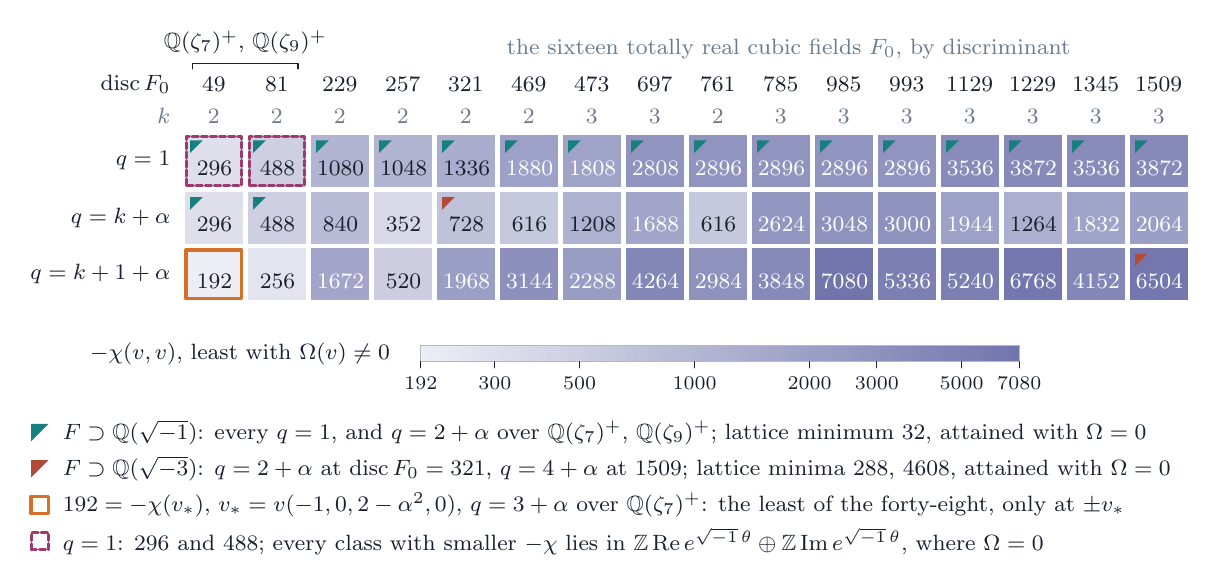
\begin{tikzpicture}[x=1cm,y=1cm,line join=round,line cap=round,
  font=\small,text=PInk,lbl/.style={inner sep=1pt}]
  \path[fill=PIndigo!17!white,draw=none] (0.0000,1.5000) rectangle (0.7400,2.1600);
  \path[fill=PIndigo!17!white,draw=none] (0.0000,0.7800) rectangle (0.7400,1.4400);
  \path[fill=PIndigo!9!white,draw=none] (0.0000,0.0600) rectangle (0.7400,0.7200);
  \path[fill=PIndigo!25!white,draw=none] (0.8000,1.5000) rectangle (1.5400,2.1600);
  \path[fill=PIndigo!25!white,draw=none] (0.8000,0.7800) rectangle (1.5400,1.4400);
  \path[fill=PIndigo!14!white,draw=none] (0.8000,0.0600) rectangle (1.5400,0.7200);
  \path[fill=PIndigo!39!white,draw=none] (1.6000,1.5000) rectangle (2.3400,2.1600);
  \path[fill=PIndigo!35!white,draw=none] (1.6000,0.7800) rectangle (2.3400,1.4400);
  \path[fill=PIndigo!47!white,draw=none] (1.6000,0.0600) rectangle (2.3400,0.7200);
  \path[fill=PIndigo!39!white,draw=none] (2.4000,1.5000) rectangle (3.1400,2.1600);
  \path[fill=PIndigo!20!white,draw=none] (2.4000,0.7800) rectangle (3.1400,1.4400);
  \path[fill=PIndigo!26!white,draw=none] (2.4000,0.0600) rectangle (3.1400,0.7200);
  \path[fill=PIndigo!43!white,draw=none] (3.2000,1.5000) rectangle (3.9400,2.1600);
  \path[fill=PIndigo!32!white,draw=none] (3.2000,0.7800) rectangle (3.9400,1.4400);
  \path[fill=PIndigo!50!white,draw=none] (3.2000,0.0600) rectangle (3.9400,0.7200);
  \path[fill=PIndigo!49!white,draw=none] (4.0000,1.5000) rectangle (4.7400,2.1600);
  \path[fill=PIndigo!29!white,draw=none] (4.0000,0.7800) rectangle (4.7400,1.4400);
  \path[fill=PIndigo!58!white,draw=none] (4.0000,0.0600) rectangle (4.7400,0.7200);
  \path[fill=PIndigo!48!white,draw=none] (4.8000,1.5000) rectangle (5.5400,2.1600);
  \path[fill=PIndigo!41!white,draw=none] (4.8000,0.7800) rectangle (5.5400,1.4400);
  \path[fill=PIndigo!52!white,draw=none] (4.8000,0.0600) rectangle (5.5400,0.7200);
  \path[fill=PIndigo!56!white,draw=none] (5.6000,1.5000) rectangle (6.3400,2.1600);
  \path[fill=PIndigo!47!white,draw=none] (5.6000,0.7800) rectangle (6.3400,1.4400);
  \path[fill=PIndigo!63!white,draw=none] (5.6000,0.0600) rectangle (6.3400,0.7200);
  \path[fill=PIndigo!56!white,draw=none] (6.4000,1.5000) rectangle (7.1400,2.1600);
  \path[fill=PIndigo!29!white,draw=none] (6.4000,0.7800) rectangle (7.1400,1.4400);
  \path[fill=PIndigo!57!white,draw=none] (6.4000,0.0600) rectangle (7.1400,0.7200);
  \path[fill=PIndigo!56!white,draw=none] (7.2000,1.5000) rectangle (7.9400,2.1600);
  \path[fill=PIndigo!55!white,draw=none] (7.2000,0.7800) rectangle (7.9400,1.4400);
  \path[fill=PIndigo!61!white,draw=none] (7.2000,0.0600) rectangle (7.9400,0.7200);
  \path[fill=PIndigo!56!white,draw=none] (8.0000,1.5000) rectangle (8.7400,2.1600);
  \path[fill=PIndigo!57!white,draw=none] (8.0000,0.7800) rectangle (8.7400,1.4400);
  \path[fill=PIndigo!72!white,draw=none] (8.0000,0.0600) rectangle (8.7400,0.7200);
  \path[fill=PIndigo!56!white,draw=none] (8.8000,1.5000) rectangle (9.5400,2.1600);
  \path[fill=PIndigo!57!white,draw=none] (8.8000,0.7800) rectangle (9.5400,1.4400);
  \path[fill=PIndigo!67!white,draw=none] (8.8000,0.0600) rectangle (9.5400,0.7200);
  \path[fill=PIndigo!60!white,draw=none] (9.6000,1.5000) rectangle (10.3400,2.1600);
  \path[fill=PIndigo!49!white,draw=none] (9.6000,0.7800) rectangle (10.3400,1.4400);
  \path[fill=PIndigo!67!white,draw=none] (9.6000,0.0600) rectangle (10.3400,0.7200);
  \path[fill=PIndigo!61!white,draw=none] (10.4000,1.5000) rectangle (11.1400,2.1600);
  \path[fill=PIndigo!42!white,draw=none] (10.4000,0.7800) rectangle (11.1400,1.4400);
  \path[fill=PIndigo!71!white,draw=none] (10.4000,0.0600) rectangle (11.1400,0.7200);
  \path[fill=PIndigo!60!white,draw=none] (11.2000,1.5000) rectangle (11.9400,2.1600);
  \path[fill=PIndigo!48!white,draw=none] (11.2000,0.7800) rectangle (11.9400,1.4400);
  \path[fill=PIndigo!63!white,draw=none] (11.2000,0.0600) rectangle (11.9400,0.7200);
  \path[fill=PIndigo!61!white,draw=none] (12.0000,1.5000) rectangle (12.7400,2.1600);
  \path[fill=PIndigo!50!white,draw=none] (12.0000,0.7800) rectangle (12.7400,1.4400);
  \path[fill=PIndigo!71!white,draw=none] (12.0000,0.0600) rectangle (12.7400,0.7200);
  \path[fill=PTeal,draw=none] (0.0700,2.0900) -- (0.2300,2.0900) -- (0.0700,1.9300) -- cycle;
  \path[fill=PTeal,draw=none] (0.0700,1.3700) -- (0.2300,1.3700) -- (0.0700,1.2100) -- cycle;
  \path[fill=PTeal,draw=none] (0.8700,2.0900) -- (1.0300,2.0900) -- (0.8700,1.9300) -- cycle;
  \path[fill=PTeal,draw=none] (0.8700,1.3700) -- (1.0300,1.3700) -- (0.8700,1.2100) -- cycle;
  \path[fill=PTeal,draw=none] (1.6700,2.0900) -- (1.8300,2.0900) -- (1.6700,1.9300) -- cycle;
  \path[fill=PTeal,draw=none] (2.4700,2.0900) -- (2.6300,2.0900) -- (2.4700,1.9300) -- cycle;
  \path[fill=PTeal,draw=none] (3.2700,2.0900) -- (3.4300,2.0900) -- (3.2700,1.9300) -- cycle;
  \path[fill=PClay,draw=none] (3.2700,1.3700) -- (3.4300,1.3700) -- (3.2700,1.2100) -- cycle;
  \path[fill=PTeal,draw=none] (4.0700,2.0900) -- (4.2300,2.0900) -- (4.0700,1.9300) -- cycle;
  \path[fill=PTeal,draw=none] (4.8700,2.0900) -- (5.0300,2.0900) -- (4.8700,1.9300) -- cycle;
  \path[fill=PTeal,draw=none] (5.6700,2.0900) -- (5.8300,2.0900) -- (5.6700,1.9300) -- cycle;
  \path[fill=PTeal,draw=none] (6.4700,2.0900) -- (6.6300,2.0900) -- (6.4700,1.9300) -- cycle;
  \path[fill=PTeal,draw=none] (7.2700,2.0900) -- (7.4300,2.0900) -- (7.2700,1.9300) -- cycle;
  \path[fill=PTeal,draw=none] (8.0700,2.0900) -- (8.2300,2.0900) -- (8.0700,1.9300) -- cycle;
  \path[fill=PTeal,draw=none] (8.8700,2.0900) -- (9.0300,2.0900) -- (8.8700,1.9300) -- cycle;
  \path[fill=PTeal,draw=none] (9.6700,2.0900) -- (9.8300,2.0900) -- (9.6700,1.9300) -- cycle;
  \path[fill=PTeal,draw=none] (10.4700,2.0900) -- (10.6300,2.0900) -- (10.4700,1.9300) -- cycle;
  \path[fill=PTeal,draw=none] (11.2700,2.0900) -- (11.4300,2.0900) -- (11.2700,1.9300) -- cycle;
  \path[fill=PTeal,draw=none] (12.0700,2.0900) -- (12.2300,2.0900) -- (12.0700,1.9300) -- cycle;
  \path[fill=PClay,draw=none] (12.0700,0.6500) -- (12.2300,0.6500) -- (12.0700,0.4900) -- cycle;
  \path[fill=none,draw=PAmber,line width=1.30pt] (0.0200,0.0800) rectangle (0.7200,0.7000);
  \path[fill=none,draw=PMag,line width=1.10pt,dash pattern=on 2.2pt off 1.1pt] (0.0200,1.5200) rectangle (0.7200,2.1400);
  \path[fill=none,draw=PMag,line width=1.10pt,dash pattern=on 2.2pt off 1.1pt] (0.8200,1.5200) rectangle (1.5200,2.1400);
  \draw[PInk,line width=0.4pt] (0.1000,3.0000) -- (0.1000,3.0700) -- (1.4400,3.0700) -- (1.4400,3.0000);
  \path[fill=PIndigo!9!white,draw=none] (3.0000,-0.7200) rectangle (3.0884,-0.5200);
  \path[fill=PIndigo!10!white,draw=none] (3.0844,-0.7200) rectangle (3.1729,-0.5200);
  \path[fill=PIndigo!11!white,draw=none] (3.1689,-0.7200) rectangle (3.2573,-0.5200);
  \path[fill=PIndigo!11!white,draw=none] (3.2533,-0.7200) rectangle (3.3418,-0.5200);
  \path[fill=PIndigo!12!white,draw=none] (3.3378,-0.7200) rectangle (3.4262,-0.5200);
  \path[fill=PIndigo!13!white,draw=none] (3.4222,-0.7200) rectangle (3.5107,-0.5200);
  \path[fill=PIndigo!14!white,draw=none] (3.5067,-0.7200) rectangle (3.5951,-0.5200);
  \path[fill=PIndigo!14!white,draw=none] (3.5911,-0.7200) rectangle (3.6796,-0.5200);
  \path[fill=PIndigo!15!white,draw=none] (3.6756,-0.7200) rectangle (3.7640,-0.5200);
  \path[fill=PIndigo!16!white,draw=none] (3.7600,-0.7200) rectangle (3.8484,-0.5200);
  \path[fill=PIndigo!16!white,draw=none] (3.8444,-0.7200) rectangle (3.9329,-0.5200);
  \path[fill=PIndigo!17!white,draw=none] (3.9289,-0.7200) rectangle (4.0173,-0.5200);
  \path[fill=PIndigo!18!white,draw=none] (4.0133,-0.7200) rectangle (4.1018,-0.5200);
  \path[fill=PIndigo!18!white,draw=none] (4.0978,-0.7200) rectangle (4.1862,-0.5200);
  \path[fill=PIndigo!19!white,draw=none] (4.1822,-0.7200) rectangle (4.2707,-0.5200);
  \path[fill=PIndigo!20!white,draw=none] (4.2667,-0.7200) rectangle (4.3551,-0.5200);
  \path[fill=PIndigo!21!white,draw=none] (4.3511,-0.7200) rectangle (4.4396,-0.5200);
  \path[fill=PIndigo!21!white,draw=none] (4.4356,-0.7200) rectangle (4.5240,-0.5200);
  \path[fill=PIndigo!22!white,draw=none] (4.5200,-0.7200) rectangle (4.6084,-0.5200);
  \path[fill=PIndigo!23!white,draw=none] (4.6044,-0.7200) rectangle (4.6929,-0.5200);
  \path[fill=PIndigo!23!white,draw=none] (4.6889,-0.7200) rectangle (4.7773,-0.5200);
  \path[fill=PIndigo!24!white,draw=none] (4.7733,-0.7200) rectangle (4.8618,-0.5200);
  \path[fill=PIndigo!25!white,draw=none] (4.8578,-0.7200) rectangle (4.9462,-0.5200);
  \path[fill=PIndigo!25!white,draw=none] (4.9422,-0.7200) rectangle (5.0307,-0.5200);
  \path[fill=PIndigo!26!white,draw=none] (5.0267,-0.7200) rectangle (5.1151,-0.5200);
  \path[fill=PIndigo!27!white,draw=none] (5.1111,-0.7200) rectangle (5.1996,-0.5200);
  \path[fill=PIndigo!28!white,draw=none] (5.1956,-0.7200) rectangle (5.2840,-0.5200);
  \path[fill=PIndigo!28!white,draw=none] (5.2800,-0.7200) rectangle (5.3684,-0.5200);
  \path[fill=PIndigo!29!white,draw=none] (5.3644,-0.7200) rectangle (5.4529,-0.5200);
  \path[fill=PIndigo!30!white,draw=none] (5.4489,-0.7200) rectangle (5.5373,-0.5200);
  \path[fill=PIndigo!30!white,draw=none] (5.5333,-0.7200) rectangle (5.6218,-0.5200);
  \path[fill=PIndigo!31!white,draw=none] (5.6178,-0.7200) rectangle (5.7062,-0.5200);
  \path[fill=PIndigo!32!white,draw=none] (5.7022,-0.7200) rectangle (5.7907,-0.5200);
  \path[fill=PIndigo!32!white,draw=none] (5.7867,-0.7200) rectangle (5.8751,-0.5200);
  \path[fill=PIndigo!33!white,draw=none] (5.8711,-0.7200) rectangle (5.9596,-0.5200);
  \path[fill=PIndigo!34!white,draw=none] (5.9556,-0.7200) rectangle (6.0440,-0.5200);
  \path[fill=PIndigo!35!white,draw=none] (6.0400,-0.7200) rectangle (6.1284,-0.5200);
  \path[fill=PIndigo!35!white,draw=none] (6.1244,-0.7200) rectangle (6.2129,-0.5200);
  \path[fill=PIndigo!36!white,draw=none] (6.2089,-0.7200) rectangle (6.2973,-0.5200);
  \path[fill=PIndigo!37!white,draw=none] (6.2933,-0.7200) rectangle (6.3818,-0.5200);
  \path[fill=PIndigo!37!white,draw=none] (6.3778,-0.7200) rectangle (6.4662,-0.5200);
  \path[fill=PIndigo!38!white,draw=none] (6.4622,-0.7200) rectangle (6.5507,-0.5200);
  \path[fill=PIndigo!39!white,draw=none] (6.5467,-0.7200) rectangle (6.6351,-0.5200);
  \path[fill=PIndigo!39!white,draw=none] (6.6311,-0.7200) rectangle (6.7196,-0.5200);
  \path[fill=PIndigo!40!white,draw=none] (6.7156,-0.7200) rectangle (6.8040,-0.5200);
  \path[fill=PIndigo!41!white,draw=none] (6.8000,-0.7200) rectangle (6.8884,-0.5200);
  \path[fill=PIndigo!42!white,draw=none] (6.8844,-0.7200) rectangle (6.9729,-0.5200);
  \path[fill=PIndigo!42!white,draw=none] (6.9689,-0.7200) rectangle (7.0573,-0.5200);
  \path[fill=PIndigo!43!white,draw=none] (7.0533,-0.7200) rectangle (7.1418,-0.5200);
  \path[fill=PIndigo!44!white,draw=none] (7.1378,-0.7200) rectangle (7.2262,-0.5200);
  \path[fill=PIndigo!44!white,draw=none] (7.2222,-0.7200) rectangle (7.3107,-0.5200);
  \path[fill=PIndigo!45!white,draw=none] (7.3067,-0.7200) rectangle (7.3951,-0.5200);
  \path[fill=PIndigo!46!white,draw=none] (7.3911,-0.7200) rectangle (7.4796,-0.5200);
  \path[fill=PIndigo!46!white,draw=none] (7.4756,-0.7200) rectangle (7.5640,-0.5200);
  \path[fill=PIndigo!47!white,draw=none] (7.5600,-0.7200) rectangle (7.6484,-0.5200);
  \path[fill=PIndigo!48!white,draw=none] (7.6444,-0.7200) rectangle (7.7329,-0.5200);
  \path[fill=PIndigo!49!white,draw=none] (7.7289,-0.7200) rectangle (7.8173,-0.5200);
  \path[fill=PIndigo!49!white,draw=none] (7.8133,-0.7200) rectangle (7.9018,-0.5200);
  \path[fill=PIndigo!50!white,draw=none] (7.8978,-0.7200) rectangle (7.9862,-0.5200);
  \path[fill=PIndigo!51!white,draw=none] (7.9822,-0.7200) rectangle (8.0707,-0.5200);
  \path[fill=PIndigo!51!white,draw=none] (8.0667,-0.7200) rectangle (8.1551,-0.5200);
  \path[fill=PIndigo!52!white,draw=none] (8.1511,-0.7200) rectangle (8.2396,-0.5200);
  \path[fill=PIndigo!53!white,draw=none] (8.2356,-0.7200) rectangle (8.3240,-0.5200);
  \path[fill=PIndigo!53!white,draw=none] (8.3200,-0.7200) rectangle (8.4084,-0.5200);
  \path[fill=PIndigo!54!white,draw=none] (8.4044,-0.7200) rectangle (8.4929,-0.5200);
  \path[fill=PIndigo!55!white,draw=none] (8.4889,-0.7200) rectangle (8.5773,-0.5200);
  \path[fill=PIndigo!56!white,draw=none] (8.5733,-0.7200) rectangle (8.6618,-0.5200);
  \path[fill=PIndigo!56!white,draw=none] (8.6578,-0.7200) rectangle (8.7462,-0.5200);
  \path[fill=PIndigo!57!white,draw=none] (8.7422,-0.7200) rectangle (8.8307,-0.5200);
  \path[fill=PIndigo!58!white,draw=none] (8.8267,-0.7200) rectangle (8.9151,-0.5200);
  \path[fill=PIndigo!58!white,draw=none] (8.9111,-0.7200) rectangle (8.9996,-0.5200);
  \path[fill=PIndigo!59!white,draw=none] (8.9956,-0.7200) rectangle (9.0840,-0.5200);
  \path[fill=PIndigo!60!white,draw=none] (9.0800,-0.7200) rectangle (9.1684,-0.5200);
  \path[fill=PIndigo!60!white,draw=none] (9.1644,-0.7200) rectangle (9.2529,-0.5200);
  \path[fill=PIndigo!61!white,draw=none] (9.2489,-0.7200) rectangle (9.3373,-0.5200);
  \path[fill=PIndigo!62!white,draw=none] (9.3333,-0.7200) rectangle (9.4218,-0.5200);
  \path[fill=PIndigo!63!white,draw=none] (9.4178,-0.7200) rectangle (9.5062,-0.5200);
  \path[fill=PIndigo!63!white,draw=none] (9.5022,-0.7200) rectangle (9.5907,-0.5200);
  \path[fill=PIndigo!64!white,draw=none] (9.5867,-0.7200) rectangle (9.6751,-0.5200);
  \path[fill=PIndigo!65!white,draw=none] (9.6711,-0.7200) rectangle (9.7596,-0.5200);
  \path[fill=PIndigo!65!white,draw=none] (9.7556,-0.7200) rectangle (9.8440,-0.5200);
  \path[fill=PIndigo!66!white,draw=none] (9.8400,-0.7200) rectangle (9.9284,-0.5200);
  \path[fill=PIndigo!67!white,draw=none] (9.9244,-0.7200) rectangle (10.0129,-0.5200);
  \path[fill=PIndigo!67!white,draw=none] (10.0089,-0.7200) rectangle (10.0973,-0.5200);
  \path[fill=PIndigo!68!white,draw=none] (10.0933,-0.7200) rectangle (10.1818,-0.5200);
  \path[fill=PIndigo!69!white,draw=none] (10.1778,-0.7200) rectangle (10.2662,-0.5200);
  \path[fill=PIndigo!70!white,draw=none] (10.2622,-0.7200) rectangle (10.3507,-0.5200);
  \path[fill=PIndigo!70!white,draw=none] (10.3467,-0.7200) rectangle (10.4351,-0.5200);
  \path[fill=PIndigo!71!white,draw=none] (10.4311,-0.7200) rectangle (10.5196,-0.5200);
  \path[fill=PIndigo!72!white,draw=none] (10.5156,-0.7200) rectangle (10.6040,-0.5200);
  \path[fill=none,draw=PRule,line width=0.35pt] (3.0000,-0.7200) rectangle (10.6000,-0.5200);
  \draw[PInk,line width=0.35pt] (3.0000,-0.7200) -- (3.0000,-0.8000);
  \draw[PInk,line width=0.35pt] (3.9402,-0.7200) -- (3.9402,-0.8000);
  \draw[PInk,line width=0.35pt] (5.0164,-0.7200) -- (5.0164,-0.8000);
  \draw[PInk,line width=0.35pt] (6.4766,-0.7200) -- (6.4766,-0.8000);
  \draw[PInk,line width=0.35pt] (7.9369,-0.7200) -- (7.9369,-0.8000);
  \draw[PInk,line width=0.35pt] (8.7911,-0.7200) -- (8.7911,-0.8000);
  \draw[PInk,line width=0.35pt] (9.8672,-0.7200) -- (9.8672,-0.8000);
  \draw[PInk,line width=0.35pt] (10.6000,-0.7200) -- (10.6000,-0.8000);
  \path[fill=PTeal,draw=none] (-1.9500,-1.5100) -- (-1.7300,-1.5100) -- (-1.9500,-1.7300) -- cycle;
  \path[fill=PClay,draw=none] (-1.9500,-1.9700) -- (-1.7300,-1.9700) -- (-1.9500,-2.1900) -- cycle;
  \path[fill=none,draw=PAmber,line width=1.30pt] (-1.9500,-2.6500) rectangle (-1.7300,-2.4300);
  \path[fill=none,draw=PMag,line width=1.10pt,dash pattern=on 2.2pt off 1.1pt] (-1.9500,-3.1100) rectangle (-1.7300,-2.8900);
  \node[lbl,text=PInk,font=\footnotesize] at (0.3800,1.7400) {$296$};
  \node[lbl,text=PInk,font=\footnotesize] at (0.3800,1.0200) {$296$};
  \node[lbl,text=PInk,font=\footnotesize] at (0.3800,0.3000) {$192$};
  \node[lbl,text=PInk,font=\footnotesize] at (1.1800,1.7400) {$488$};
  \node[lbl,text=PInk,font=\footnotesize] at (1.1800,1.0200) {$488$};
  \node[lbl,text=PInk,font=\footnotesize] at (1.1800,0.3000) {$256$};
  \node[lbl,text=PInk,font=\footnotesize] at (1.9800,1.7400) {$1080$};
  \node[lbl,text=PInk,font=\footnotesize] at (1.9800,1.0200) {$840$};
  \node[lbl,text=white,font=\footnotesize] at (1.9800,0.3000) {$1672$};
  \node[lbl,text=PInk,font=\footnotesize] at (2.7800,1.7400) {$1048$};
  \node[lbl,text=PInk,font=\footnotesize] at (2.7800,1.0200) {$352$};
  \node[lbl,text=PInk,font=\footnotesize] at (2.7800,0.3000) {$520$};
  \node[lbl,text=PInk,font=\footnotesize] at (3.5800,1.7400) {$1336$};
  \node[lbl,text=PInk,font=\footnotesize] at (3.5800,1.0200) {$728$};
  \node[lbl,text=white,font=\footnotesize] at (3.5800,0.3000) {$1968$};
  \node[lbl,text=white,font=\footnotesize] at (4.3800,1.7400) {$1880$};
  \node[lbl,text=PInk,font=\footnotesize] at (4.3800,1.0200) {$616$};
  \node[lbl,text=white,font=\footnotesize] at (4.3800,0.3000) {$3144$};
  \node[lbl,text=white,font=\footnotesize] at (5.1800,1.7400) {$1808$};
  \node[lbl,text=PInk,font=\footnotesize] at (5.1800,1.0200) {$1208$};
  \node[lbl,text=white,font=\footnotesize] at (5.1800,0.3000) {$2288$};
  \node[lbl,text=white,font=\footnotesize] at (5.9800,1.7400) {$2808$};
  \node[lbl,text=white,font=\footnotesize] at (5.9800,1.0200) {$1688$};
  \node[lbl,text=white,font=\footnotesize] at (5.9800,0.3000) {$4264$};
  \node[lbl,text=white,font=\footnotesize] at (6.7800,1.7400) {$2896$};
  \node[lbl,text=PInk,font=\footnotesize] at (6.7800,1.0200) {$616$};
  \node[lbl,text=white,font=\footnotesize] at (6.7800,0.3000) {$2984$};
  \node[lbl,text=white,font=\footnotesize] at (7.5800,1.7400) {$2896$};
  \node[lbl,text=white,font=\footnotesize] at (7.5800,1.0200) {$2624$};
  \node[lbl,text=white,font=\footnotesize] at (7.5800,0.3000) {$3848$};
  \node[lbl,text=white,font=\footnotesize] at (8.3800,1.7400) {$2896$};
  \node[lbl,text=white,font=\footnotesize] at (8.3800,1.0200) {$3048$};
  \node[lbl,text=white,font=\footnotesize] at (8.3800,0.3000) {$7080$};
  \node[lbl,text=white,font=\footnotesize] at (9.1800,1.7400) {$2896$};
  \node[lbl,text=white,font=\footnotesize] at (9.1800,1.0200) {$3000$};
  \node[lbl,text=white,font=\footnotesize] at (9.1800,0.3000) {$5336$};
  \node[lbl,text=white,font=\footnotesize] at (9.9800,1.7400) {$3536$};
  \node[lbl,text=white,font=\footnotesize] at (9.9800,1.0200) {$1944$};
  \node[lbl,text=white,font=\footnotesize] at (9.9800,0.3000) {$5240$};
  \node[lbl,text=white,font=\footnotesize] at (10.7800,1.7400) {$3872$};
  \node[lbl,text=PInk,font=\footnotesize] at (10.7800,1.0200) {$1264$};
  \node[lbl,text=white,font=\footnotesize] at (10.7800,0.3000) {$6768$};
  \node[lbl,text=white,font=\footnotesize] at (11.5800,1.7400) {$3536$};
  \node[lbl,text=white,font=\footnotesize] at (11.5800,1.0200) {$1832$};
  \node[lbl,text=white,font=\footnotesize] at (11.5800,0.3000) {$4152$};
  \node[lbl,text=white,font=\footnotesize] at (12.3800,1.7400) {$3872$};
  \node[lbl,text=white,font=\footnotesize] at (12.3800,1.0200) {$2064$};
  \node[lbl,text=white,font=\footnotesize] at (12.3800,0.3000) {$6504$};
  \node[lbl,anchor=east,text=PInk,font=\footnotesize] at (-0.1400,1.8300) {$q=1$};
  \node[lbl,anchor=east,text=PInk,font=\footnotesize] at (-0.1400,1.1100) {$q=k+\alpha$};
  \node[lbl,anchor=east,text=PInk,font=\footnotesize] at (-0.1400,0.3900) {$q=k+1+\alpha$};
  \node[lbl,text=PSlate,font=\footnotesize] at (0.3700,2.4000) {$2$};
  \node[lbl,text=PInk,font=\footnotesize] at (0.3700,2.8000) {$49$};
  \node[lbl,text=PSlate,font=\footnotesize] at (1.1700,2.4000) {$2$};
  \node[lbl,text=PInk,font=\footnotesize] at (1.1700,2.8000) {$81$};
  \node[lbl,text=PSlate,font=\footnotesize] at (1.9700,2.4000) {$2$};
  \node[lbl,text=PInk,font=\footnotesize] at (1.9700,2.8000) {$229$};
  \node[lbl,text=PSlate,font=\footnotesize] at (2.7700,2.4000) {$2$};
  \node[lbl,text=PInk,font=\footnotesize] at (2.7700,2.8000) {$257$};
  \node[lbl,text=PSlate,font=\footnotesize] at (3.5700,2.4000) {$2$};
  \node[lbl,text=PInk,font=\footnotesize] at (3.5700,2.8000) {$321$};
  \node[lbl,text=PSlate,font=\footnotesize] at (4.3700,2.4000) {$2$};
  \node[lbl,text=PInk,font=\footnotesize] at (4.3700,2.8000) {$469$};
  \node[lbl,text=PSlate,font=\footnotesize] at (5.1700,2.4000) {$3$};
  \node[lbl,text=PInk,font=\footnotesize] at (5.1700,2.8000) {$473$};
  \node[lbl,text=PSlate,font=\footnotesize] at (5.9700,2.4000) {$3$};
  \node[lbl,text=PInk,font=\footnotesize] at (5.9700,2.8000) {$697$};
  \node[lbl,text=PSlate,font=\footnotesize] at (6.7700,2.4000) {$2$};
  \node[lbl,text=PInk,font=\footnotesize] at (6.7700,2.8000) {$761$};
  \node[lbl,text=PSlate,font=\footnotesize] at (7.5700,2.4000) {$3$};
  \node[lbl,text=PInk,font=\footnotesize] at (7.5700,2.8000) {$785$};
  \node[lbl,text=PSlate,font=\footnotesize] at (8.3700,2.4000) {$3$};
  \node[lbl,text=PInk,font=\footnotesize] at (8.3700,2.8000) {$985$};
  \node[lbl,text=PSlate,font=\footnotesize] at (9.1700,2.4000) {$3$};
  \node[lbl,text=PInk,font=\footnotesize] at (9.1700,2.8000) {$993$};
  \node[lbl,text=PSlate,font=\footnotesize] at (9.9700,2.4000) {$3$};
  \node[lbl,text=PInk,font=\footnotesize] at (9.9700,2.8000) {$1129$};
  \node[lbl,text=PSlate,font=\footnotesize] at (10.7700,2.4000) {$3$};
  \node[lbl,text=PInk,font=\footnotesize] at (10.7700,2.8000) {$1229$};
  \node[lbl,text=PSlate,font=\footnotesize] at (11.5700,2.4000) {$3$};
  \node[lbl,text=PInk,font=\footnotesize] at (11.5700,2.8000) {$1345$};
  \node[lbl,text=PSlate,font=\footnotesize] at (12.3700,2.4000) {$3$};
  \node[lbl,text=PInk,font=\footnotesize] at (12.3700,2.8000) {$1509$};
  \node[lbl,anchor=east,text=PSlate,font=\footnotesize] at (-0.1400,2.4000) {$k$};
  \node[lbl,anchor=east,text=PInk,font=\footnotesize] at (-0.1400,2.8000) {$\operatorname{disc}F_{0}$};
  \node[lbl,anchor=south,text=PInk,font=\footnotesize] at (0.7700,3.1400) {$\QQ(\zeta_{7})^{+}$, $\QQ(\zeta_{9})^{+}$};
  \node[lbl,text=PSlate,font=\footnotesize] at (7.6700,3.2500) {the sixteen totally real cubic fields $F_{0}$, by discriminant};
  \node[lbl,anchor=north,text=PInk,font=\scriptsize] at (3.0000,-0.8700) {$192$};
  \node[lbl,anchor=north,text=PInk,font=\scriptsize] at (3.9402,-0.8700) {$300$};
  \node[lbl,anchor=north,text=PInk,font=\scriptsize] at (5.0164,-0.8700) {$500$};
  \node[lbl,anchor=north,text=PInk,font=\scriptsize] at (6.4766,-0.8700) {$1000$};
  \node[lbl,anchor=north,text=PInk,font=\scriptsize] at (7.9369,-0.8700) {$2000$};
  \node[lbl,anchor=north,text=PInk,font=\scriptsize] at (8.7911,-0.8700) {$3000$};
  \node[lbl,anchor=north,text=PInk,font=\scriptsize] at (9.8672,-0.8700) {$5000$};
  \node[lbl,anchor=north,text=PInk,font=\scriptsize] at (10.6000,-0.8700) {$7080$};
  \node[lbl,anchor=east,text=PInk,font=\footnotesize] at (2.6500,-0.6200) {$-\chi(v,v)$, least with $\Omega(v)\neq0$};
  \node[lbl,anchor=west,text=PInk,font=\footnotesize] at (-1.5900,-1.6200) {$F\supset\QQ(\sqrt{-1})$: every $q=1$, and $q=2+\alpha$ over $\QQ(\zeta_{7})^{+}$, $\QQ(\zeta_{9})^{+}$; lattice minimum $32$, attained with $\Omega=0$};
  \node[lbl,anchor=west,text=PInk,font=\footnotesize] at (-1.5900,-2.0800) {$F\supset\QQ(\sqrt{-3})$: $q=2+\alpha$ at $\operatorname{disc}F_{0}=321$, $q=4+\alpha$ at $1509$; lattice minima $288$, $4608$, attained with $\Omega=0$};
  \node[lbl,anchor=west,text=PInk,font=\footnotesize] at (-1.5900,-2.5400) {$192=-\chi(v_{*})$, $v_{*}=v(-1,0,2-\alpha^{2},0)$, $q=3+\alpha$ over $\QQ(\zeta_{7})^{+}$: the least of the forty-eight, only at $\pm v_{*}$};
  \node[lbl,anchor=west,text=PInk,font=\footnotesize] at (-1.5900,-3.0000) {$q=1$: $296$ and $488$; every class with smaller $-\chi$ lies in $\ZZ\operatorname{Re}e^{\sqrt{-1}\,\theta}\oplus\ZZ\operatorname{Im}e^{\sqrt{-1}\,\theta}$, where $\Omega=0$};
\end{tikzpicture}
\end{document}
